\subsubsection{word2vec} % (fold)
\label{sub:own_word2vec}
Besides offering implementations of Latent Semantic Analysis and LDA, the aforementioned \textit{gensim} library\,\cite{gensim_python} also implements the word2vec tool created by Mikolov et al. and is recommended for the generation of word embeddings in a review on NLP toolkits performed in 2018\,\cite{solangi_review_2018}.

We then followed different approaches, for the creation of our desired word embeddings. First, we tried to train our own model from the requiremnent senteces given the \crowdre{} dataset both with and without prior processing of the requirements through our NLP pipeline and on both architectures.\\
Being unsatisfied with the outcome, in a second attempt we created our embeddings using a pre-trained word2vec model, which contained the word vectors of a model trained on about 100 billion words of the Google News dataset\footnote{\url{https://code.google.com/archive/p/word2vec/}, last visited 2020-01-19}. Even though the outcome was different, the underlying workflow for both approaches was very similiar once the trained model was available:
\begin{itemize}
	\item For every tokenized requirement sentence, create a sentence matrix by replacing every word by its vector representation:\\
	$reqtokens = \{"As", "smart", "home", "owner", \dots\}$\\
	$embeddings = \{ \vec{as}, \vec{smart}, \vec{home}, \vec{owner}, \dots \}$
	\item On the resulting matrices, reduce the different x-dimensions to the dimension of the shortest sentence using Principal Component Analysis
	\item Use K-Means to generate a number of clusters on these now equally shaped matrices
	\item Visualize the results by transforming the data into 2d space using t-SNE\cite{maaten_visualizing_2008}
\end{itemize}


\begin{figure}[ht]
  \begin{center}
    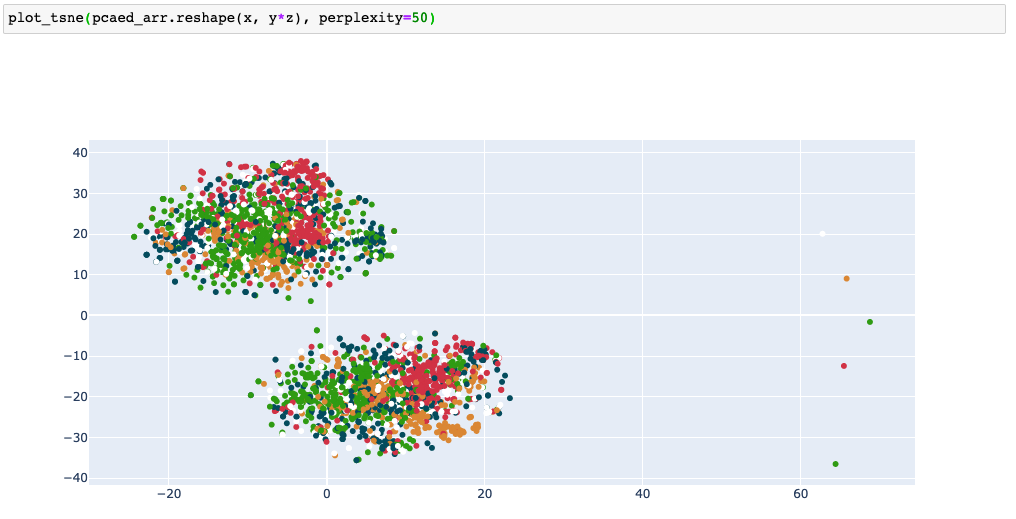
\includegraphics[width=\textwidth]{screenshots/google_word_2_vec_tsne_opti4.png}
    \caption{word2vec result of the clustering with a pretrained model (plotted with t-SNE)}
    \label{fig:w2v-pretrained-4}
  \end{center}
\end{figure}
\FloatBarrier